\documentclass[12pt,a4paper]{article}
	%[fleqn] %%% --to make all equation left-algned--

% \usepackage[utf8]{inputenc}
% \DeclareUnicodeCharacter{1D12A}{\doublesharp}
% \DeclareUnicodeCharacter{2693}{\anchor}
% \usepackage{dingbat}
% \DeclareRobustCommand\dash\unskip\nobreak\thinspace{\textemdash\allowbreak\thinspace\ignorespaces}
\usepackage[top=2in, bottom=1in, left=1in, right=1in]{geometry}
%\usepackage{fullpage}

\usepackage{fancyhdr}\pagestyle{fancy}\rhead{Stephanie Wang}\lhead{EE236B homework 8}

\usepackage{amsmath,amssymb,amsthm,amsfonts,microtype,stmaryrd}
	%{mathtools,wasysym,yhmath}

\usepackage[usenames,dvipsnames]{xcolor}
\newcommand{\blue}[1]{\textcolor{blue}{#1}}
\newcommand{\red}[1]{\textcolor{red}{#1}}
\newcommand{\gray}[1]{\textcolor{gray}{#1}}
\newcommand{\fgreen}[1]{\textcolor{ForestGreen}{#1}}

\usepackage{mdframed}
	%\newtheorem{mdexample}{Example}
	\definecolor{warmgreen}{rgb}{0.8,0.9,0.85}
	% --Example:
	% \begin{center}
	% \begin{minipage}{0.7\textwidth}
	% \begin{mdframed}[backgroundcolor=warmgreen, 
	% skipabove=4pt,skipbelow=4pt,hidealllines=true, 
	% topline=false,leftline=false,middlelinewidth=10pt, 
	% roundcorner=10pt] 
	%%%% --CONTENTS-- %%%%
	% \end{mdframed}\end{minipage}\end{center}	

\usepackage{graphicx} \graphicspath{{}}
	% --Example:
	% \includegraphics[scale=0.5]{picture name}
%\usepackage{caption} %%% --some awful package to make caption...

\usepackage{hyperref}\hypersetup{linktocpage,colorlinks}\hypersetup{citecolor=black,filecolor=black,linkcolor=black,urlcolor=blue,breaklinks=true}

%%% --Text Fonts
%\usepackage{times} %%% --Times New Roman for LaTeX
%\usepackage{fontspec}\setmainfont{Times New Roman} %%% --Times New Roman; XeLaTeX only

%%% --Math Fonts
\renewcommand{\v}[1]{\ifmmode\mathbf{#1}\fi}
%\renewcommand{\mbf}[1]{\mathbf{#1}} %%% --vector
%\newcommand{\ca}[1]{\mathcal{#1}} %%% --"bigO"
%\newcommand{\bb}[1]{\mathbb{#1}} %%% --"Natural, Real numbers"
%\newcommand{\rom}[1]{\romannumeral{#1}} %%% --Roman numbers

%%% --Quick Arrows
\newcommand{\ra}[1]{\ifnum #1=1\rightarrow\fi\ifnum #1=2\Rightarrow\fi\ifnum #1=3\Rrightarrow\fi\ifnum #1=4\rightrightarrows\fi\ifnum #1=5\rightleftarrows\fi\ifnum #1=6\mapsto\fi\ifnum #1=7\iffalse\fi\fi\ifnum #1=8\twoheadrightarrow\fi\ifnum #1=9\rightharpoonup\fi\ifnum #1=0\rightharpoondown\fi}

%\newcommand{\la}[1]{\ifnum #1=1\leftarrow\fi\ifnum #1=2\Leftarrow\fi\ifnum #1=3\Lleftarrow\fi\ifnum #1=4\leftleftarrows\fi\ifnum #1=5\rightleftarrows\fi\ifnum #1=6\mapsfrom\ifnum #1=7\iffalse\fi\fi\ifnum #1=8\twoheadleftarrow\fi\ifnum #1=9\leftharpoonup\fi\ifnum #1=0\leftharpoondown\fi}

%\newcommand{\ua}[1]{\ifnum #1=1\uparrow\fi\ifnum #1=2\Uparrow\fi}
%\newcommand{\da}[1]{\ifnum #1=1\downarrow\fi\ifnum #1=2\Downarrow\fi}

%%% --Special Editor Config
\renewcommand{\ni}{\noindent}
\newcommand{\onum}[1]{\raisebox{.5pt}{\textcircled{\raisebox{-1pt} {#1}}}}

\newcommand{\claim}[1]{\underline{``{#1}":}}

\renewcommand{\l}{\left}\renewcommand{\r}{\right}

\newcommand{\casebrak}[4]{\left \{ \begin{array}{ll} {#1},&{#2}\\{#3},&{#4} \end{array} \right.}
%\newcommand{\ttm}[4]{\l[\begin{array}{cc}{#1}&{#2}\\{#3}&{#4}\end{array}\r]} %two-by-two-matrix
%\newcommand{\tv}[2]{\l[\begin{array}{c}{#1}\\{#2}\end{array}\r]}

\def\dps{\displaystyle}

\let\italiccorrection=\/
\def\/{\ifmmode\expandafter\frac\else\italiccorrection\fi}


%%% --General Math Symbols
\def\bc{\because}
\def\tf{\therefore}

%%% --Frequently used OPERATORS shorthand
\newcommand{\INT}[2]{\int_{#1}^{#2}}
% \newcommand{\UPINT}{\bar\int}
% \newcommand{\UPINTRd}{\overline{\int_{\bb R ^d}}}
\newcommand{\SUM}[2]{\sum\limits_{#1}^{#2}}
\newcommand{\PROD}[2]{\prod\limits_{#1}^{#2}}
\newcommand{\CUP}[2]{\bigcup\limits_{#1}^{#2}}
\newcommand{\CAP}[2]{\bigcap\limits_{#1}^{#2}}
% \newcommand{\SUP}[1]{\sup\limits_{#1}}
% \newcommand{\INF}[1]{\inf\limits_{#1}}
\DeclareMathOperator*{\argmin}{arg\,min}
\DeclareMathOperator*{\argmax}{arg\,max}
\newcommand{\pd}[2]{\frac{\partial{#1}}{\partial{#2}}}
\def\tr{\text{tr}}

\renewcommand{\o}{\circ}
\newcommand{\x}{\times}
\newcommand{\ox}{\otimes}

\newcommand\ie{{\it i.e. }}
\newcommand\wrt{{w.r.t. }}
\newcommand\dom{\mathbf{dom\:}}

%%% --Frequently used VARIABLES shorthand
\def\R{\ifmmode\mathbb R\fi}
\def\N{\ifmmode\mathbb N\fi}
\renewcommand{\O}{\mathcal{O}}

\newcommand{\dt}{\Delta t}
\def\vA{\mathbf{A}}
\def\vB{\mathbf{B}}\def\cB{\mathcal{B}}
\def\vC{\mathbf{C}}
\def\vD{\mathbf{D}}
\def\vE{\mathbf{E}}
\def\vF{\mathbf{F}}\def\tvF{\tilde{\mathbf{F}}}
\def\vG{\mathbf{G}}
\def\vH{\mathbf{H}}
\def\vI{\mathbf{I}}\def\cI{\mathcal{I}}
\def\vJ{\mathbf{J}}
\def\vK{\mathbf{K}}
\def\vL{\mathbf{L}}\def\cL{\mathcal{L}}
\def\vM{\mathbf{M}}
\def\vN{\mathbf{N}}\def\cN{\mathcal{N}}
\def\vO{\mathbf{O}}
\def\vP{\mathbf{P}}
\def\vQ{\mathbf{Q}}
\def\vR{\mathbf{R}}
\def\vS{\mathbf{S}}
\def\vT{\mathbf{T}}
\def\vU{\mathbf{U}}
\def\vV{\mathbf{V}}
\def\vW{\mathbf{W}}
\def\vX{\mathbf{X}}
\def\vY{\mathbf{Y}}
\def\vZ{\mathbf{Z}}

\def\va{\mathbf{a}}
\def\vb{\mathbf{b}}
\def\vc{\mathbf{c}}
\def\vd{\mathbf{d}}
\def\ve{\mathbf{e}}
\def\vf{\mathbf{f}}
\def\vg{\mathbf{g}}
\def\vh{\mathbf{h}}
\def\vi{\mathbf{i}}
\def\vj{\mathbf{j}}
\def\vk{\mathbf{k}}
\def\vl{\mathbf{l}}
\def\vm{\mathbf{m}}
\def\vn{\mathbf{n}}
\def\vo{\mathbf{o}}
\def\vp{\mathbf{p}}
\def\vq{\mathbf{q}}
\def\vr{\mathbf{r}}
\def\vs{\mathbf{s}}
\def\vt{\mathbf{t}}
\def\vu{\mathbf{u}}
\def\vv{\mathbf{v}}\def\tvv{\tilde{\mathbf{v}}}
\def\vw{\mathbf{w}}
\def\vx{\mathbf{x}}\def\tvx{\tilde{\mathbf{x}}}
\def\vy{\mathbf{y}}
\def\vz{\mathbf{z}}

%%% --Numerical analysis related
%\newcommand{\nxt}{^{n+1}}
%\newcommand{\pvs}{^{n-1}}
%\newcommand{\hfnxt}{^{n+\frac12}}

%%%%%%%%%%%%%%%%%%%%%%%%%%%%%%%%%%%%%%%%%%%%%%%%%%%%%%%%%%%%%%%%%%%%%%%%%%%%%%%%%%%%%%%%%%%%%%%%%%%%%%%%%%%%%%%%%%%%%%%%%%%%%%%%%%%%%%%%%%%%%%%%%%%%%%%%%%%%%%%%%%%%%%%%%%%%%%%%%%%%%%%%%%%%%%%%%%%%%%
\begin{document}
\subsubsection*{Exercise 5.18 [Boyd \& Vandenberghe, 2004]}
{\it Ans:}  Without any sophisticated thoughts the problem is equivalent to the feasibility problem
\begin{align*}
\mbox{minimize\;\;\;}& 1\\
\mbox{subject to\;\;}& \inf \{a^Tx \mid Ax\preceq b\} > \gamma > \sup\{a^Ty \mid Cy \preceq d\} \\
\mbox{variable\;\;\;}& a, \gamma
\end{align*}
Consider $s^\ast$ as the optimal value of the below problem
\begin{align*}
\mbox{minimize\;\;\;}& a^Tx\\
\mbox{subject to\;\;}& Ax\preceq b\\
\mbox{variable\;\;\;}& x
\end{align*}
The Lagrangian $L(x, \lambda) = a^Tx + \lambda^T(Ax-b)$ gives the Lagrange dual function
$$g(\lambda) = \casebrak{-\lambda^Tb}{A^T\lambda + a = 0}{-\infty}{\mbox{else}}$$
We should be able to assume the polyhedron $\mathcal P_1$ has nonempty interior, that is, Slater's condition for this problem, hence strong duality gives $s^\ast = -\lambda^Tb$ for some $\lambda \succeq 0$ and $A^T\lambda + a = 0$. Similarly if $t^\ast$ is the optimal value of the below problem
\begin{align*}
\mbox{maximize\;\;\;}& a^Ty\\
\mbox{subject to\;\;}& Cy\preceq d\\
\mbox{variable\;\;\;}& y
\end{align*}
The Lagrangian $L(y, \mu) = -a^Ty + \mu^T(Cy-d)$ gives the Lagrange dual function
$$g(\mu) = \casebrak{-\mu^Td}{C^T\mu - a = 0}{-\infty}{\mbox{else}}$$
With the same assumption that $\mathcal P_2$ has nonempty interior, $t^\ast = -\mu^Td$ for some $\mu \succeq 0$ and $C^T\mu-a = 0$. The original problem can be viewed as
\begin{align*}
\mbox{minimize\;\;\;} &1\\
\mbox{subject to\;\;} & -\lambda^Tb > \gamma > -\mu^Td\\
& \lambda \succeq 0, \mu \succeq 0\\
& A^T\lambda + a = 0\\
& C^T\mu - a = 0
\end{align*}
which is an LP feasibility problem now. \qed

\newpage\subsubsection*{Additional Exercise 4.25 [Boyd \& Vandenberghe, 2017]}
{\it Ans:} The first equality follows from
$$D_1AD_2u = diag(u) diag(Ax)^{-1}Adiag(u)^{-1}diag(x)u = diag(u)diag(Ax)^{-1}Ax = u$$
To derive a equivalent convex problem, first take logarithm to the objective and constraints,
\begin{align*}
\mbox{minimize\;\;\;} & -\SUM{i=1}n\alpha_i \log (Ax)_i \\
\mbox{subject to\;\;} & \SUM{i=1}n \alpha_i \log x_i = 0 \\
& x \succ 0
\end{align*}
The Lagrangian and the optimality conditions are
\begin{align*}
L(x, \lambda, \nu) &= -\alpha^T \log(Ax) -\lambda^T x + \nu\alpha^T \log x\\
\nabla_xL(x,\lambda, \nu) &= -A^T diag(Ax)^{-1} \alpha -\lambda + \nu diag(x)^{-1}\alpha = 0
\end{align*}
Here $\log(\cdot)$ denotes the element-wise logarithm on vectors. The complementary slackness on $x\succ0$ ensures that $\lambda =0$. The condition above gives 
$$-diag(x)A^Tdiag(Ax)^{-1}\alpha + \nu \alpha = 0 $$
If we sum over the entries of this vector equality, we get
\begin{align*}
0 &= -\SUM{i=1}nx_i\l(\SUM{j=1}n a_{ji}\/{\alpha_j}{y_j}\r) + \nu \SUM{i=1}n \alpha_i \\
&= -\SUM{i=1}n \SUM{j=1}n \/{\alpha_j a_{ji}x_i}{y_j} + \nu\SUM{i=1}n\alpha_i \\
&= -\SUM{j=1}n \/{\alpha_j}{y_j}\SUM{i=1}na_{ji}x_i + \nu\SUM{i=1}n\alpha_i \\
&= -\SUM{j=1}n \/{\alpha_j}{y_j} y_j + \nu\SUM{i=1}n \alpha_i \\
&= (-1 + \nu)\SUM{i=1}n \alpha_i
\end{align*}
and $\nu = 0$. This gives us $A^Tdiag(y)^{-1}\alpha = diag(x)^{-1}\alpha$, or, $A^Tdiag(y)^{-1}diag(u)v = diag(x)^{-1}diag(u)v$ since $\alpha_i = u_iv_i$. The equality we are aiming for is 
$$(diag(u) diag(y)^{-1} A diag(u)^{-1} diag(x))^T v = v$$
now naturally follows. \qed




\newpage\subsubsection*{Additional Exercise 4.26 [Boyd \& Vandenberghe, 2017]}
{\it Ans:} (a) Use the fact that $\|\cdot\|_2^\ast = \|\cdot\|_2, \|\cdot\|_1^\ast = \|\cdot\|_\infty$ and the Legendre transform of the norms, we derive the Lagrange dual function
\begin{align*}
g(\nu) &= \inf_{x, y} L(x, y, \nu)\\
&= \inf_{x, y} \|y\|_2 + \gamma \|x\|_1 + \nu^T(Ax-b-y) \\
&= -\nu^Tb + \l(\inf_y \|y\|_2 - \nu^Ty\r) + \l(\inf_x \gamma \|x\|_1 + \nu^TAx\r) \\
&= -\nu^Tb -\l(\sup_y y^T\nu - \|y\|_2 \r) - \gamma \l(\sup_x  x^T\l(-\/1\gamma A^T\nu\r)- \|x\|_1\r)\\
&= \casebrak{-\nu^Tb}{\|\nu\|_2^\ast \leq 1, \l\|-\/1\gamma A^T\nu\r\|_1^\ast \leq 1}{-\infty}{\mbox{else}} \\
&= \casebrak{-\nu^Tb}{\|\nu\|_2 \leq 1, \l\|A^T\nu\r\|_\infty \leq \gamma}{-\infty}{\mbox{else}}
\end{align*}
(b) From the aspects of the equivalent problem, $y^\ast = Ax^\ast - b \neq 0$ and $r = y/\|y\|_2$. The KKT condition suggests
$$\nabla_yL(x^\ast, y^\ast, \nu^\ast) = \frac{y^\ast}{\|y^\ast\|_2} -\nu = 0$$
Hence we see $\nu^\ast = r$ here. Since $\nu^\ast$ is feasible for the dual problem, we have $\|A^Tr\|_\infty  = \|A^T\nu^\ast\|_\infty \leq \gamma$. The other KKT condition requires
\begin{align*}
\nabla_yL(x^\ast, y^\ast, \nu^\ast) & = \gamma sgn(x^\ast) + A^T \nu^\ast\\
&= \gamma sgn(x^\ast) + A^Tr = 0
\end{align*}
Hence $r^T Ax^\ast + \gamma \|x^\ast\|_1 = (\nabla_xL(x^\ast, y^\ast, \nu^\ast))^Tx^\ast = 0$. \\
\\
(c) The KKT condition on $\nabla_yL$ from part (b) asserts
$$a_i^Tr = -\gamma sgn(x^\ast_i)$$
where $a_i$ denotes the $i$-th column of $A$. Suppose $\|a_i\|_2 < \gamma$, then by Cauchy's inequality $a_i^Tr < \gamma$ (since $r$ is defined to be an unit vector) and the above equality cannot hold unless $sgn(x^\ast_i) = 0$, \ie $x^\ast_i = 0$. \qed


\newpage\subsubsection*{Additional Exercise 6.5 [Boyd \& Vandenberghe, 2017]}
{\it Ans:} (a) The maximum likelihood estimate of $x$ is 
$$x = \argmax \PROD{i=1}m p(\phi^{-1}(y_i) -a_i^Tx)$$
where $p(t) = \/1{\sqrt{2\pi\sigma^2}} e^{-\/{t^2}{2\sigma^2}}$ is the p.d.f. of the IID's $v_i \sim \mathcal N(0, \sigma^2)$. To find a convex representation of this problem we can take logarithm to the objective function and get $f_0(x) = \SUM{i=1}m\l( -\/12\log(2\pi\sigma^2) - \/{(\phi^{-1}(y_i) - a_i^Tx)^2}{2\sigma^2} \r)$, or we can drop the constant $-\/m2 \log(2\pi\sigma^2)$ and let 
\begin{align*}
f_0(x) & = -\/1{2\sigma^2}\SUM{i=1}n (\phi^{-1}(y_i) - a_i^Tx)^2\\
&= -\/1{2\sigma^2} \|z - A^Tx\|_2^2
\end{align*}
where $A = [a_1, \cdots, a_m]$ is the collection of the coefficient vectors. This is a least square minimization problem except that $z$ is another variable with some inequality constraint inscribed due to $\alpha \leq \phi'(u) \leq \beta$. In particular, from mean value theorem, $\frac{y_i - y_j}{z_i-z_j} = \phi'(\xi_{ij})$ for any $i, j = 1, \cdots, m$, we get the induced inequalities
$$\/{y_i-y_j}\beta\leq z_i-z_j \leq \/{y_i-y_j}{\alpha}$$
for $y_i > y_j$. Now assume $y$ is sorted that $y_{k+1} \geq y_k$, the problem to be solved can be formulated as below
\begin{align*}
\mbox{minimize\;\;\;} & \|A^Tx - z\|_2^2 \\
\mbox{subject to\;\;} & \frac{y_{k+1}-y_k}\beta\leq z_{k+1}-z_k \leq \/{y_{k+1}-y_k}{\alpha}\mbox{ for } k = 1, \cdots, m-1
\end{align*}
Note that if it happens $y_{k+1} = y_k$, then $z_{k+1} = z_k$ will be enforced! \\
\\
(b) The following plot is the optimal solution $z$ versus $y$. 
\begin{center}
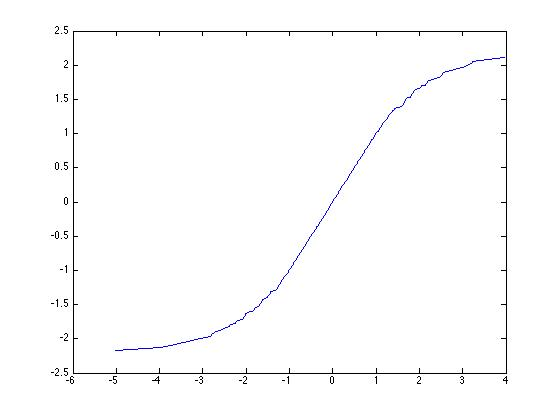
\includegraphics[scale=0.4]{hw8P65.jpg}
\end{center}
Attached is the code to inscribe the problem and call CVX. 
\begin{verbatim}
D = zeros(299,300);
for k=1:299
    D(k,k) = -1;
    D(k,k+1) = 1;
end

cvx_begin
variables x(4) z(300)
minimize norm(A*x - z)
subject to 
    (1/beta)*D*y <= D*z
    D*z <= (1/alpha)*D*y
cvx_end
\end{verbatim}
Here's some numerics from the result.
\begin{verbatim}
Calling SDPT3 4.0: 899 variables, 305 equality constraints
   For improved efficiency, SDPT3 is solving the dual problem.
------------------------------------------------------------

 num. of constraints = 305
 dim. of socp   var  = 301,   num. of socp blk  =  1
 dim. of linear var  = 598
 20 linear variables from unrestricted variable.
 *** convert ublk to lblk
*******************************************************************
   SDPT3: Infeasible path-following algorithms
*******************************************************************
 version  predcorr  gam  expon  scale_data
    NT      1      0.000   1        0    
it pstep dstep pinfeas dinfeas  gap      prim-obj      dual-obj    cputime
-------------------------------------------------------------------
 0|0.000|0.000|8.2e+00|5.9e+01|7.1e+05| 5.037923e+03  0.000000e+00| 0:0:00| chol  1  1 
 1|0.885|0.977|9.4e-01|1.6e+00|2.4e+04| 4.812382e+03 -1.693377e+01| 0:0:01| chol  1  1 
 2|0.684|0.627|3.0e-01|6.6e-01|1.1e+04| 3.665563e+03 -2.905354e+01| 0:0:01| chol  1  1 
 3|0.923|0.369|2.3e-02|4.3e-01|5.3e+03| 1.970508e+03 -3.497857e+01| 0:0:01| chol  1  1 
 4|0.874|0.338|2.9e-03|2.9e-01|3.0e+03| 1.229351e+03 -3.654966e+01| 0:0:01| chol  1  1 
 5|0.973|0.730|7.7e-05|7.9e-02|6.8e+02| 3.949011e+02 -3.017530e+01| 0:0:01| chol  1  1 
 6|0.604|0.204|3.1e-05|6.3e-02|4.8e+02| 3.024580e+02 -2.742389e+01| 0:0:01| chol  1  1 
 7|1.000|0.218|7.8e-07|4.9e-02|2.6e+02| 1.689486e+02 -2.408657e+01| 0:0:01| chol  1  1 
 8|0.730|0.535|3.8e-07|2.3e-02|1.3e+02| 9.771440e+01 -1.625992e+01| 0:0:01| chol  1  1 
 9|1.000|0.261|6.7e-08|1.7e-02|6.7e+01| 4.575721e+01 -1.366559e+01| 0:0:01| chol  1  1 
10|0.823|0.455|2.7e-08|9.2e-03|3.6e+01| 2.368631e+01 -1.011086e+01| 0:0:01| chol  1  1 
11|0.967|0.351|6.3e-09|6.0e-03|1.8e+01| 9.156954e+00 -7.802653e+00| 0:0:01| chol  1  1 
12|1.000|0.384|2.5e-09|3.7e-03|1.0e+01| 4.238214e+00 -5.807395e+00| 0:0:01| chol  1  1 
13|0.736|0.354|1.2e-09|2.4e-03|7.1e+00| 2.320164e+00 -4.583437e+00| 0:0:01| chol  1  1 
14|0.563|0.288|6.9e-10|1.7e-03|5.5e+00| 1.608416e+00 -3.780771e+00| 0:0:01| chol  1  1 
15|0.727|0.281|2.2e-10|1.2e-03|3.6e+00| 2.221933e-01 -3.263875e+00| 0:0:01| chol  1  1 
16|0.900|0.283|5.2e-10|8.7e-04|2.4e+00|-5.236924e-01 -2.851653e+00| 0:0:01| chol  1  1 
17|0.908|0.329|3.1e-10|5.9e-04|1.6e+00|-9.046204e-01 -2.467141e+00| 0:0:01| chol  1  1 
18|0.742|0.475|1.2e-10|3.1e-04|8.7e-01|-1.177404e+00 -2.033419e+00| 0:0:01| chol  1  1 
19|0.807|0.238|6.2e-11|2.4e-04|6.4e-01|-1.289185e+00 -1.913648e+00| 0:0:01| chol  1  1 
20|0.875|0.389|1.9e-10|1.4e-04|3.8e-01|-1.377674e+00 -1.752529e+00| 0:0:01| chol  1  1 
21|1.000|0.325|5.8e-11|9.7e-05|2.5e-01|-1.421602e+00 -1.665739e+00| 0:0:01| chol  1  1 
22|0.640|0.547|5.2e-11|4.4e-05|1.2e-01|-1.440453e+00 -1.558271e+00| 0:0:01| chol  1  1 
23|0.789|0.149|2.5e-11|3.7e-05|1.0e-01|-1.447220e+00 -1.545533e+00| 0:0:01| chol  1  1 
24|1.000|0.291|3.7e-11|2.7e-05|7.2e-02|-1.452773e+00 -1.523698e+00| 0:0:01| chol  1  1 
25|0.926|0.436|9.0e-11|2.3e-05|4.2e-02|-1.458300e+00 -1.498800e+00| 0:0:01| chol  1  1 
26|1.000|0.901|4.0e-13|1.0e-05|7.8e-03|-1.460940e+00 -1.468540e+00| 0:0:01| chol  1  1 
27|1.000|0.774|1.0e-13|2.0e-06|2.4e-03|-1.462750e+00 -1.465152e+00| 0:0:01| chol  1  1 
28|0.908|0.936|1.6e-13|6.0e-07|7.3e-04|-1.463201e+00 -1.463925e+00| 0:0:01| chol  1  1 
29|1.000|0.972|1.6e-13|1.8e-07|7.2e-05|-1.463545e+00 -1.463615e+00| 0:0:01| chol  1  1 
30|1.000|0.965|3.7e-13|1.8e-08|7.6e-06|-1.463575e+00 -1.463583e+00| 0:0:02| chol  1  1 
31|1.000|0.974|1.5e-12|1.9e-09|7.9e-07|-1.463579e+00 -1.463579e+00| 0:0:02| chol  1  1 
32|0.998|0.988|9.6e-13|1.9e-10|1.5e-08|-1.463579e+00 -1.463579e+00| 0:0:02|
  stop: max(relative gap, infeasibilities) < 1.49e-08
-------------------------------------------------------------------
 number of iterations   = 32
 primal objective value = -1.46357893e+00
 dual   objective value = -1.46357895e+00
 gap := trace(XZ)       = 1.54e-08
 relative gap           = 3.92e-09
 actual relative gap    = 3.34e-09
 rel. primal infeas (scaled problem)   = 9.61e-13
 rel. dual     "        "       "      = 1.95e-10
 rel. primal infeas (unscaled problem) = 0.00e+00
 rel. dual     "        "       "      = 0.00e+00
 norm(X), norm(y), norm(Z) = 9.4e+00, 2.4e+01, 8.6e+00
 norm(A), norm(b), norm(C) = 5.2e+01, 2.0e+00, 1.0e+01
 Total CPU time (secs)  = 1.58  
 CPU time per iteration = 0.05  
 termination code       =  0
 DIMACS: 9.6e-13  0.0e+00  5.5e-10  0.0e+00  3.3e-09  3.9e-09
-------------------------------------------------------------------
 
------------------------------------------------------------
Status: Solved
Optimal value (cvx_optval): +1.46358

>> max((D*y) ./ (D*z))

ans =

    1.0000

>> min((D*y) ./ (D*z))

ans =

     0

>> x

x =

    0.4819
   -0.4657
    0.9364
    0.9297

\end{verbatim}

\newpage\subsubsection*{Additional Exercise 7.1 [Boyd \& Vandenberghe, 2017]}
{\it Ans:} (a) Suppose $a_i^TQa_i \leq 1$ for $i=1,\cdots,p$. For $x\in\R^n$ with $x^TQ^{-1}x\leq 1$, or, say, $\|Q^{-1/2}x\|_2^2 \leq 1$, Cauchy's inequality gives
$$|a_i^Tx| = |(Q^{1/2}a_i)^T (Q^{-1/2}x)| \leq \|Q^{1/2}a_i\|_2 = \sqrt{a_i^TQa_i} \leq 1$$
for $i=1,\cdots, p$. On the other hand suppose $|a_i^Tx|\leq 1$ for $i=1,\cdots, p$ whenever $x^TQ^{-1}x \leq 1$. Introduce a new variable $y = Q^{-1/2}x$, then the assumed condition states 
$$\|y\|_2^2 \leq 1 \ra2 |(Q^{1/2}a_i)^T y|\leq 1 \mbox{ for } i = 1,\cdots, p$$
If $a_j^TQa_j > 1$ for some $j$, then take $y_j = Q^{1/2}a_j / \|Q^{1/2}a_j\|_2$, we can violate the above predicate since $\|y_j\|_2^2 = 1$ yet 
$$|(Q^{1/2}a_j)^T y_j| = \|Q^{1/2}a_j\| = \sqrt{a_j^TQa_j} > 1$$
(b) Denote $A = [a_1, \cdots, a_p] \in \R^{n\x p}$ be the collection of coefficients of the constraints. We first derive the Lagrange dual function from the Lagrangian and the Legendre transform of log-determinant,
\begin{align*}
L(Q, \lambda) &= \log \det Q^{-1} + \SUM{i=1}p \lambda_i(a_i^TQa_i - 1)\\
&= \log \det Q^{-1} + diag(\lambda) : (A^TQA) - \mathbf1^T\lambda\\
&= -\mathbf1^T\lambda - \l((-Adiag(\lambda)A^T) : Q - \log \det Q^{-1}\r)\\
g(\lambda) &= \inf_Q L(Q, \lambda) \\
&= -\mathbf1^T\lambda - \log\det(-Adiag(\lambda)A^T)^{-1} + n \\
&= n -\mathbf1^T\lambda - \log\det\l(-\SUM{i=1}p \lambda_ia_ia_i^T\r)^{-1}
\end{align*}
under the (domain) assumption $-Adiag(\lambda)A^T = -\SUM{i=1}p \lambda_ia_ia_i^T\prec 0$. The dual problem can be formulated now, 
\begin{align*}
\mbox{maximize\;\;\;} & n -\mathbf1^T\lambda - \log\det\l(-Adiag(\lambda)A^T \r)^{-1} \\
\mbox{subject to\;\;} & Adiag(\lambda)A^T \succ 0 \\
& \lambda \succeq 0
\end{align*}
Note here that 
(c) The KKT condition suggests 
\begin{align*}
\nabla_Q L(Q, \lambda) &= 0\\
&= -Q^{-1} + Adiag(\lambda)A^T
\end{align*}
Hence $Q = (Adiag(\lambda)A^T)^{-1}$. Now for $x\in C$, \ie $|a_i^Tx|\leq 1$ for $i=1,\cdots, p$, 
$$x^TQ^{-1}x = x^TAdiag(\lambda)A^Tx = \SUM{i=1}p\lambda_i z_i^2$$
where $z = A^Tx \preceq \mathbf1$ since $|z_i|  = |a_i^Tx|\leq 1$. On the other hand, due to the strong duality, $d^\ast = p^\ast$, 
$$n - \mathbf1^T\lambda - \log\det Q = \log\det Q^{-1}$$
$$n - \mathbf1^T\lambda = \log\det Q + \log\det Q^{-1} = \log (\det Q \det Q^{-1}) = \log\det I = 0 $$
therefore,
$$x^T Q^{-1}x = \SUM{i=1}p \lambda_i z_i^2 \leq \SUM{i=1}p \lambda_i = \mathbf1^T\lambda = n$$\qed

\end{document}



